\section{Protótipo de Interface}
O protótipo de interface para a aplicação foi feito com o \textit{Pencil}, ferramenta aconselhada pelos docentes da UC.

A página inicial do programa é a pagina de login.
\begin{center}
 	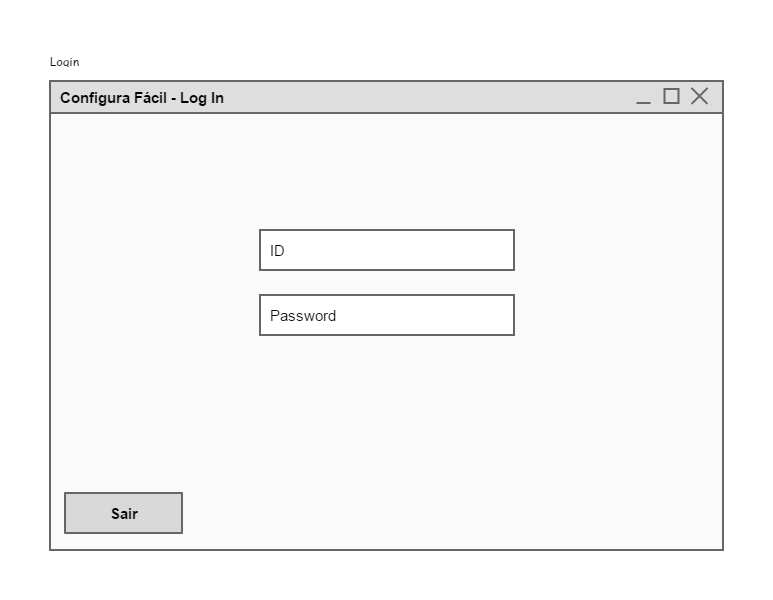
\includegraphics[width = 5in]{Prototipagem/configura_fcil_root.png}
\end{center}

Daqui, o utilizador pode ir para uma das seguintes janelas, dependendo do seu estatuto na aplicação:

\begin{center}
 	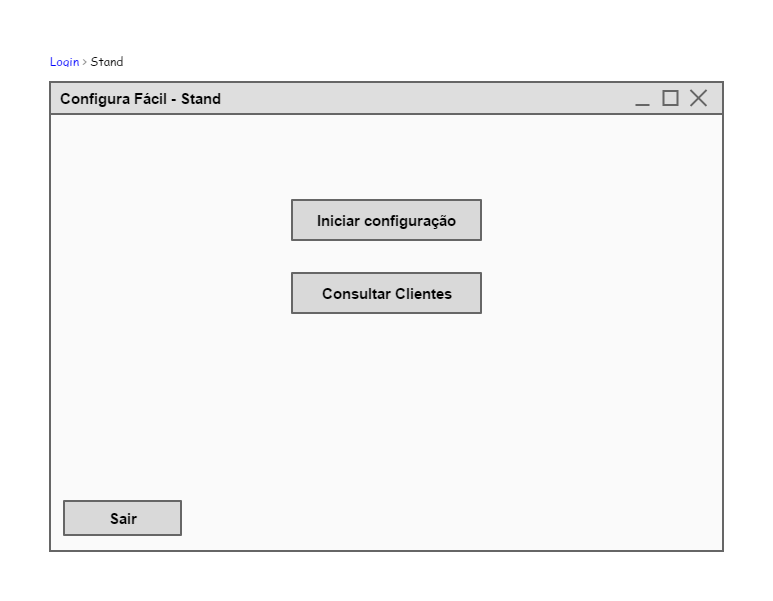
\includegraphics[width = 5.5in]{Prototipagem/configura_fcil_stand.png}

 	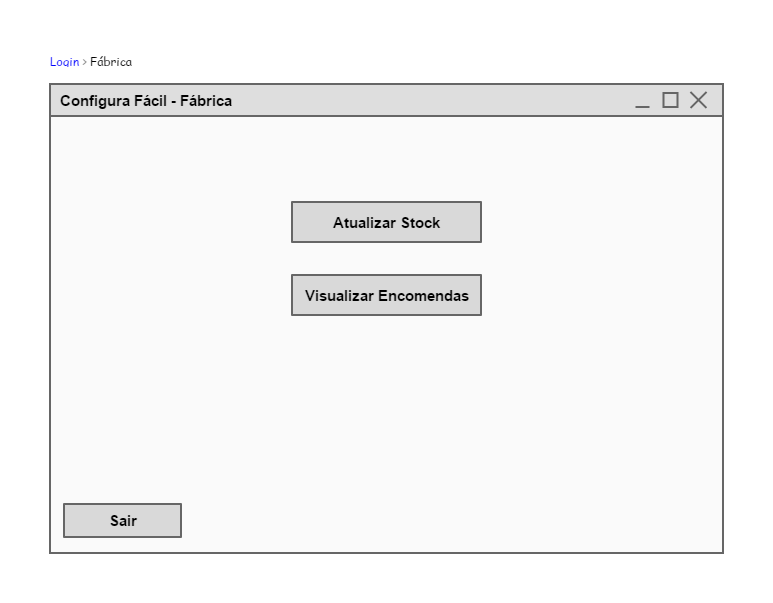
\includegraphics[width = 5.5in]{Prototipagem/configura_fcil_fbrica.png}

 	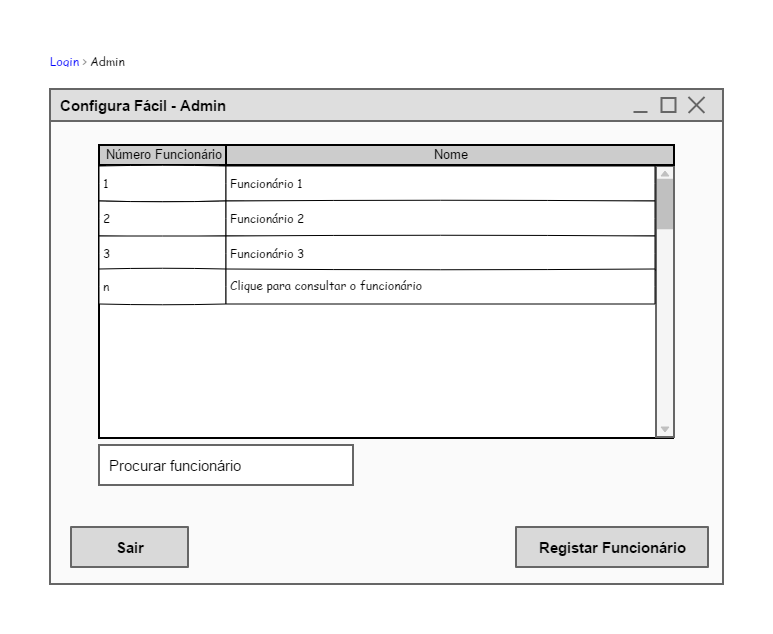
\includegraphics[width = 5.5in]{Prototipagem/configura_fcil_admin.png}
\end{center}


A partir da janela do Stand encontramos a seguinte interface:
\begin{center}
 	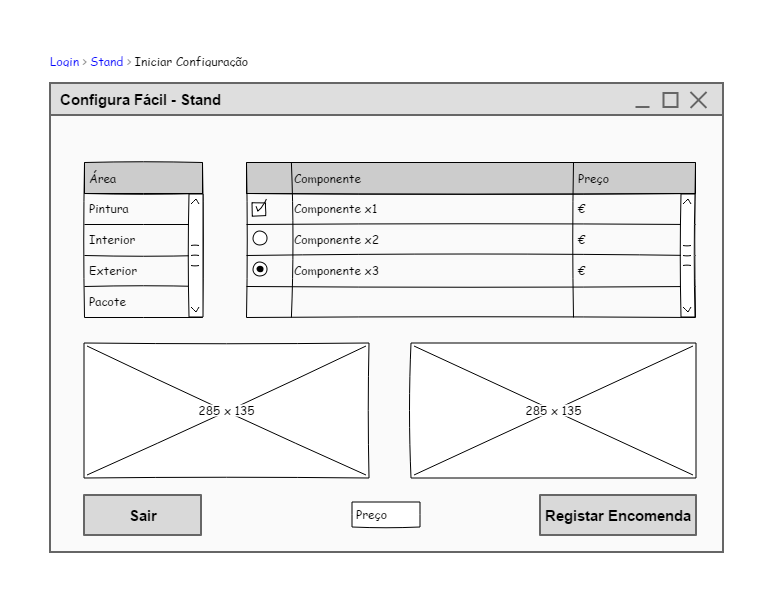
\includegraphics[width = 5in]{Prototipagem/configurao_de_carro.png}

 	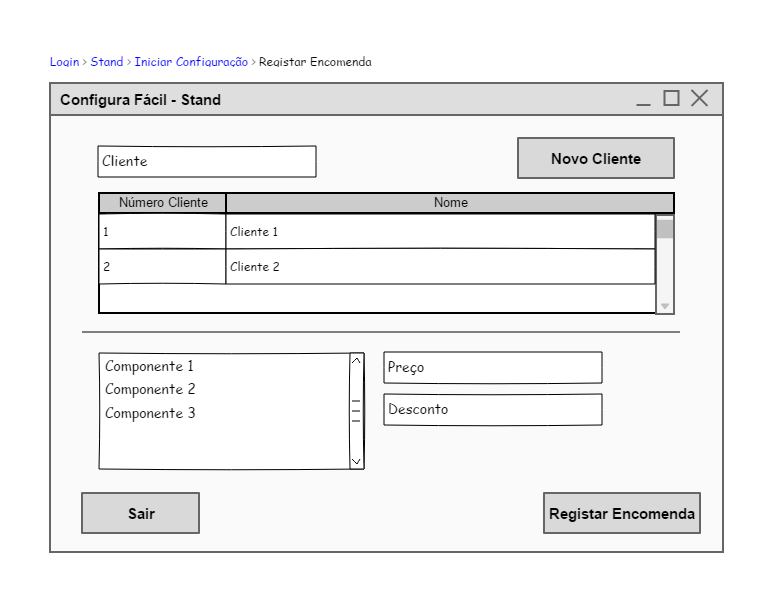
\includegraphics[width = 5.5in]{Prototipagem/registar_encomenda.png}

 	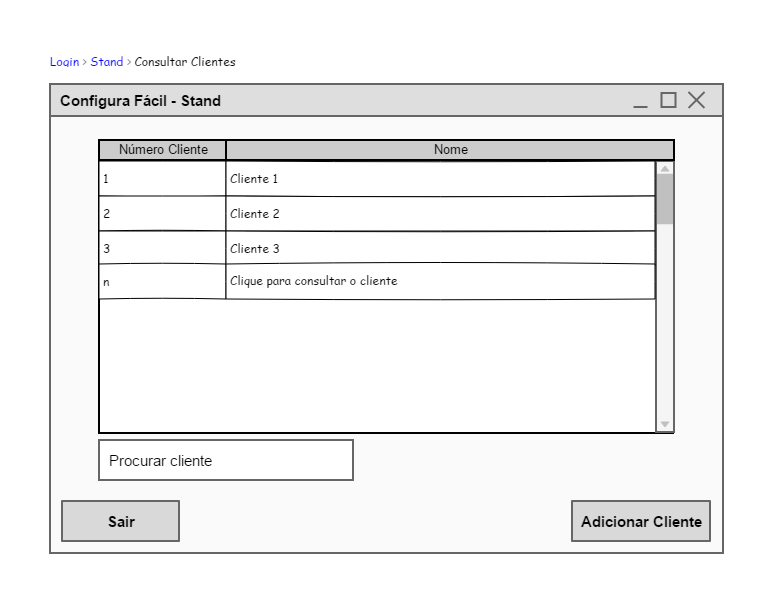
\includegraphics[width = 5.5in]{Prototipagem/consultar_clientes.png}
	
	\begin{table}[]
		\begin{tabular}{cc}
 			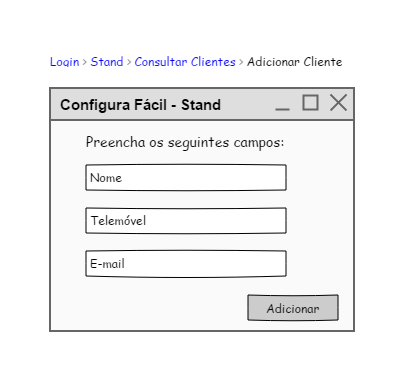
\includegraphics[width = 3in]{Prototipagem/adicionar_cliente.png}	& 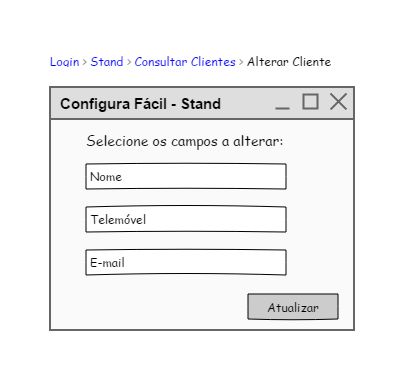
\includegraphics[width = 3in]{Prototipagem/alterar_cliente.png}
		\end{tabular}
	\end{table}
 	 	
\end{center}

Já quando o utilizador é um gestor da fábrica, a interface gráfica que o guiará pela aplicação é a seguinte:
\begin{center}
	\begin{table}[!htbp]
		\begin{tabular}{cc}
 			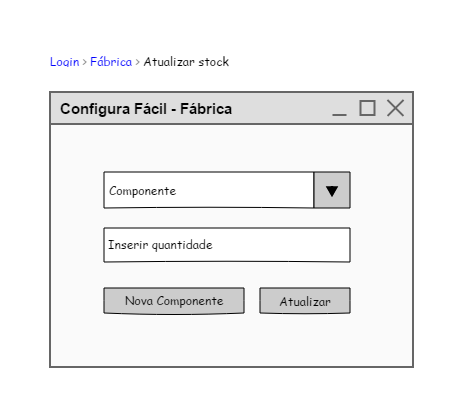
\includegraphics[width = 3in]{Prototipagem/atualizar_stock.png} & 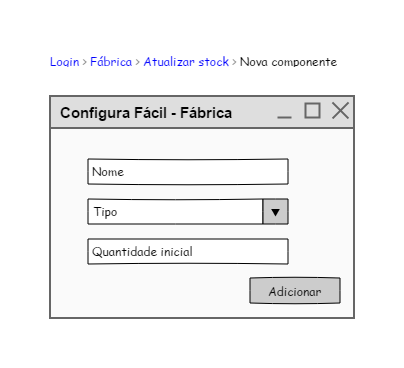
\includegraphics[width = 3in]{Prototipagem/nova_componente.png}
		\end{tabular}
	\end{table}

 	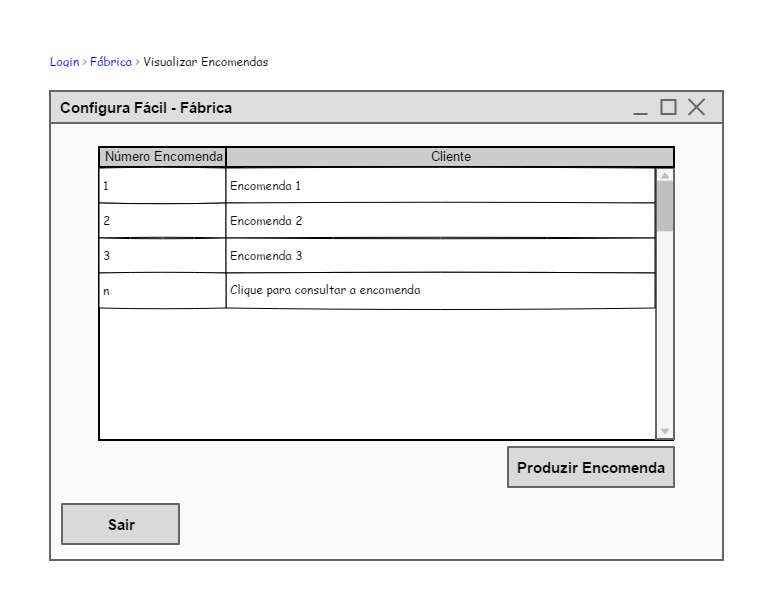
\includegraphics[width = 5.5in]{Prototipagem/visualizar_encomendas.png}

\end{center}

Por fim, quando o funcionário faz o Login como Admistrador será esta a sua visão da aplicação:
\begin{center}
	\begin{table}[!htbp]
		\begin{tabular}{cc}
 			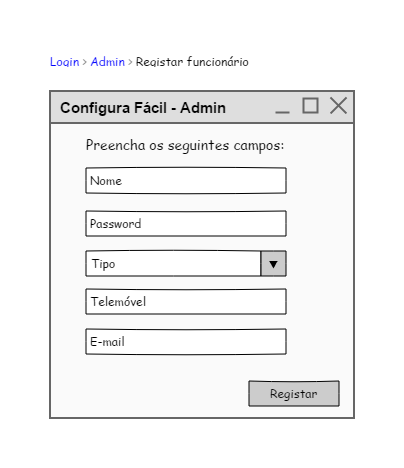
\includegraphics[width = 3in]{Prototipagem/registar_funcionrio.png} & 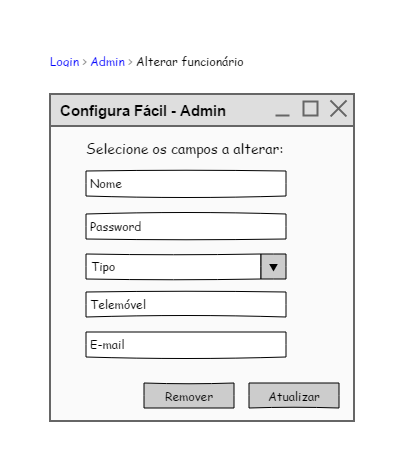
\includegraphics[width = 3in]{Prototipagem/alterar_funcionrio.png}
		\end{tabular}
	\end{table}

\end{center}